\subsection{Event yields}\label{sswwupgrade:results_yields}
After applying the full event selection, the analysis is broken down into four channels based off of the flavor of the signal leptons: $\mu\mu$, $ee$, $\mu e$, and $e\mu$.
The full signal and background event yields are shown in Table~\ref{tab:sswwupgrade_yields_default} for each channel separately and combined using the default event selection.
3489 EWK \ssww events are expected compared to 9900 background events.
The dominant sources of background are jets faking electrons followed by charge misidentification and diboson processes.
Triboson events, QCD \ssww, and other non-prompt sources make up approximately 5\% of the total background combined.

\begin{table}[htbp]
  \centering
  \begin{tabular}{l|c|cccc}
    ~ 				& All channels 	& $\mu\mu$ & $ee$ & $\mu e$ & $e\mu$  \\
    \hline\hline
    \ssww (QCD) & 206.4 & 91.1 & 22.8 & 38.4 & 54.1\\
    Charge Misidentification & 2300 & 0.0 & 2100 & 90 & 160\\
    Jets faking electrons & 5000 & 0.0 & 3400 & 1200 & 340\\
    $WZ+ZZ$ & 2040 & 500 & 438 & 423 & 680\\
    Tribosons & 115 & 47 & 15.4 & 21.6 & 31.2\\
    Other non-prompt & 210 & 110 & 20 & 60 & 27\\
    \hline
    Total Background & 9900 & 750 & 6000 & 1900 & 1290\\
    Signal \ssww (EWK) & 3489 & 1435 & 432 & 679 & 944\\
    \hline
  \end{tabular}
  \caption{Signal and background event yields using the default event selection for an integrated luminosity of $\mathcal{L} = 3000~\textrm{fb}^{-1}$. Events containing a fake or charge-flipped electron are removed from their respective sources and combined into a single entry each.} 
  \label{tab:sswwupgrade_yields_default}
\end{table}

The event yields for the optimized selection detailed in Section~\ref{sswwupgrade:opt_results} are listed in Table~\ref{tab:sswwupgrade_yields_optimized}.
After optimization, 2958 signal events and just 2310 background events are expected.
Diboson events are now the primary source of background, as the optimization greatly reduces the fake and charge mis-ID contributions.
As discussed earlier, the increase in the leading and subleading jet $\pt$ cuts as well as the loosening of the centrality cut are most responsible for the changes in the signal and background yields; distributions of these quantities using the default and the optimized event selections can be found in Figures~\ref{fig:sswwupgrade_jet0pt_compare}, \ref{fig:sswwupgrade_jet1pt_compare}, and \ref{fig:sswwupgrade_centrality_compare}, respectively.

\begin{table}[htbp]
  \centering
  \begin{tabular}{l|c|cccc}
    ~ 				& All channels 	& $\mu\mu$ & $ee$ & $\mu e$ & $e\mu$  \\
    \hline\hline
    \ssww (QCD) & 168.7 & 74.6 & 19.7 & 32.2 & 42.2\\
    Charge Misidentification & 200 & 0.0 & 11 & 30 & 160\\
    Jets faking electrons & 460 & 0.0 & 130 & 260 & 70\\
    $WZ+ZZ$ & 1286 & 322 & 289 & 271 & 404\\
    Tribosons & 76 & 30.1 & 9.6 & 15.1 & 21.6\\
    Other non-prompt & 120 & 29 & 16.6 & 50 & 19\\
    \hline
    Total Background & 2310 & 455 & 480 & 660 & 710\\
    Signal \ssww (EWK) & 2958 & 1228 & 380 & 589 & 761\\
    \hline
  \end{tabular}
  \caption{Signal and background event yields using the optimized event selection for an integrated luminosity of $\mathcal{L} = 3000~\textrm{fb}^{-1}$. Events containing a fake or charge-flipped electron are removed from their respective sources and combined into a single entry each.} 
  \label{tab:sswwupgrade_yields_optimized}
\end{table}

\begin{figure}[htbp]
  \centering
  \begin{subfigure}[b]{.48\textwidth}
    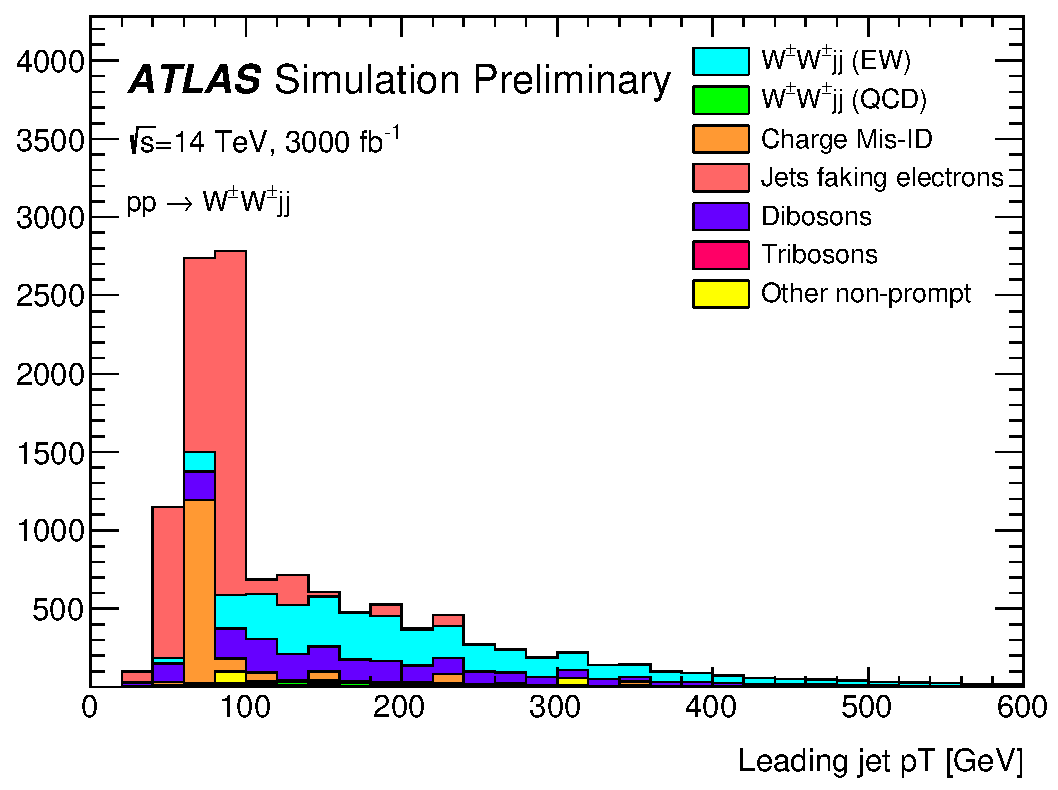
\includegraphics[width=\textwidth]{figs/ssww_upgrade/distributions/default/all_pass9_jet0_pt-cropped}
    \caption{Default selection}
    \label{fig:sswwupgrade_jet0pt_compare_d}
  \end{subfigure}
  \begin{subfigure}[b]{.474\textwidth}
  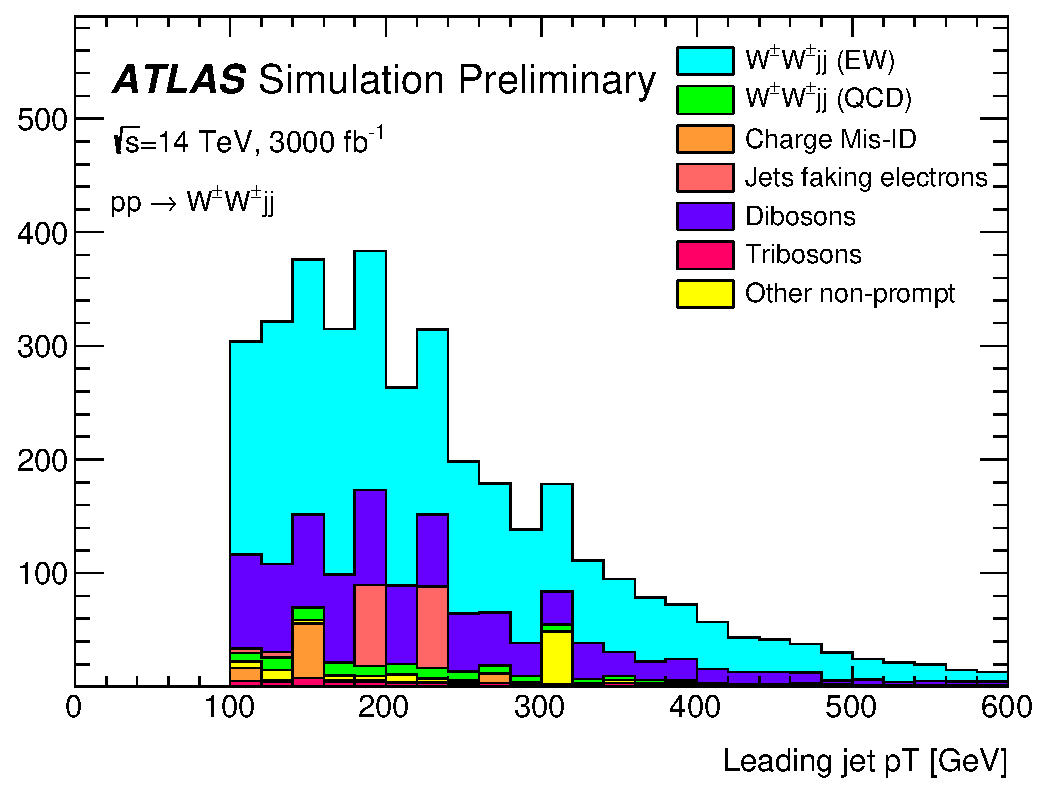
\includegraphics[width=\textwidth]{figs/ssww_upgrade/distributions/optimized/all_pass9_jet0_pt-cropped}
    \caption{Optimized selection}
    \label{fig:sswwupgrade_jet0pt_compare_o}
  \end{subfigure}
  \caption{$\pt$ distributions for the leading jet using the default (left) and optimized (right) event selections for all channels combined.}
  \label{fig:sswwupgrade_jet0pt_compare}
\end{figure}

\begin{figure}[htbp]
  \centering
  \begin{subfigure}[b]{.48\textwidth}
    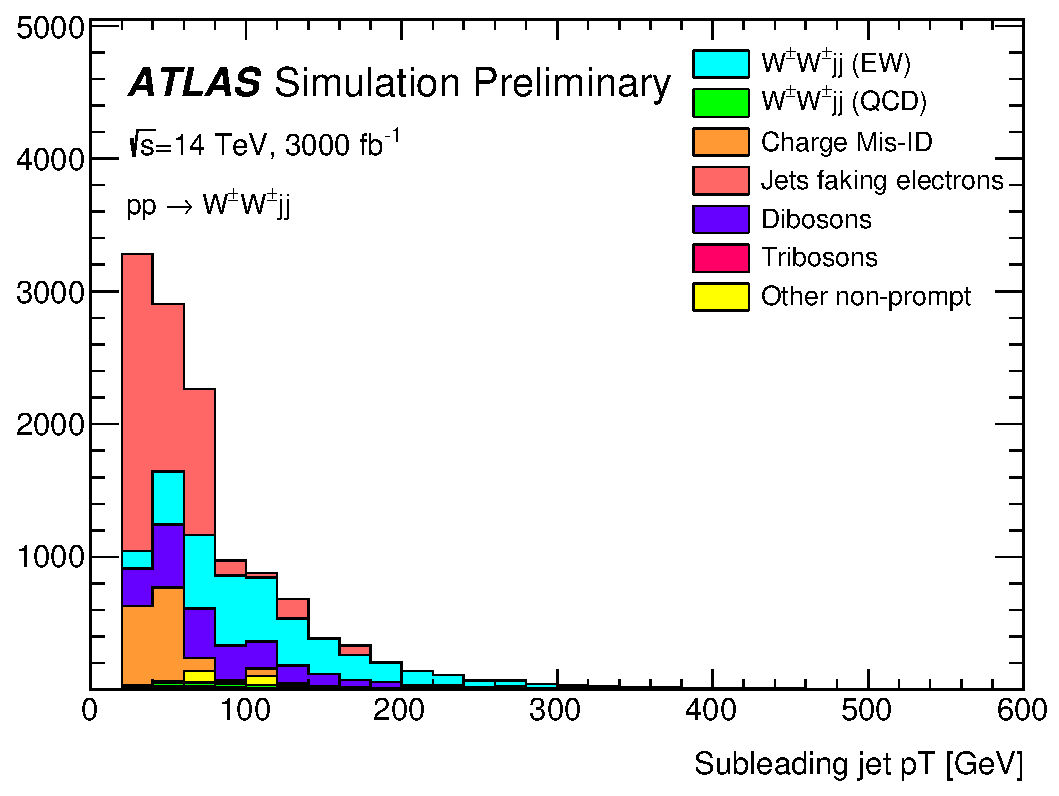
\includegraphics[width=\textwidth]{figs/ssww_upgrade/distributions/default/all_pass9_jet1_pt-cropped}
    \caption{Default selection}
    \label{fig:sswwupgrade_jet1pt_compare_d}
  \end{subfigure}
  \begin{subfigure}[b]{.475\textwidth}
  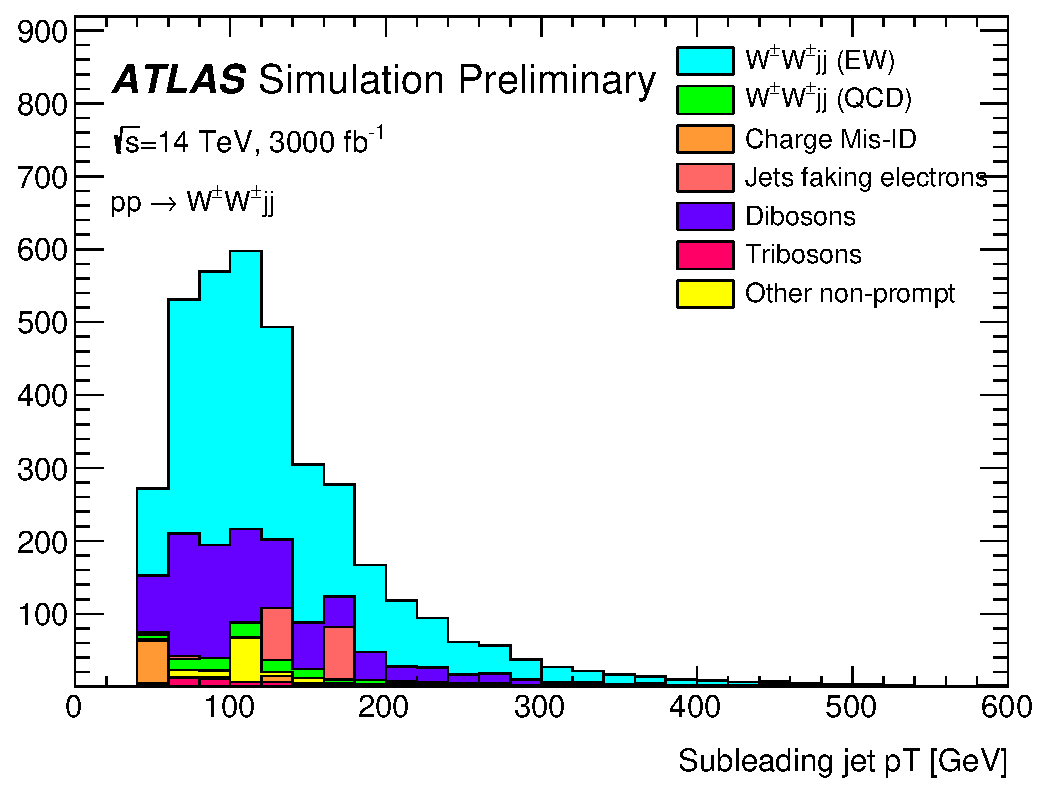
\includegraphics[width=\textwidth]{figs/ssww_upgrade/distributions/optimized/all_pass9_jet1_pt-cropped}
    \caption{Optimized selection}
    \label{fig:sswwupgrade_jet1pt_compare_o}
  \end{subfigure}
  \caption{$\pt$ distributions for the subleading jet using the default (left) and optimized (right) event selections for all channels combined.}
  \label{fig:sswwupgrade_jet1pt_compare}
\end{figure}

\begin{figure}[htbp]
  \centering
  \begin{subfigure}[b]{.48\textwidth}
    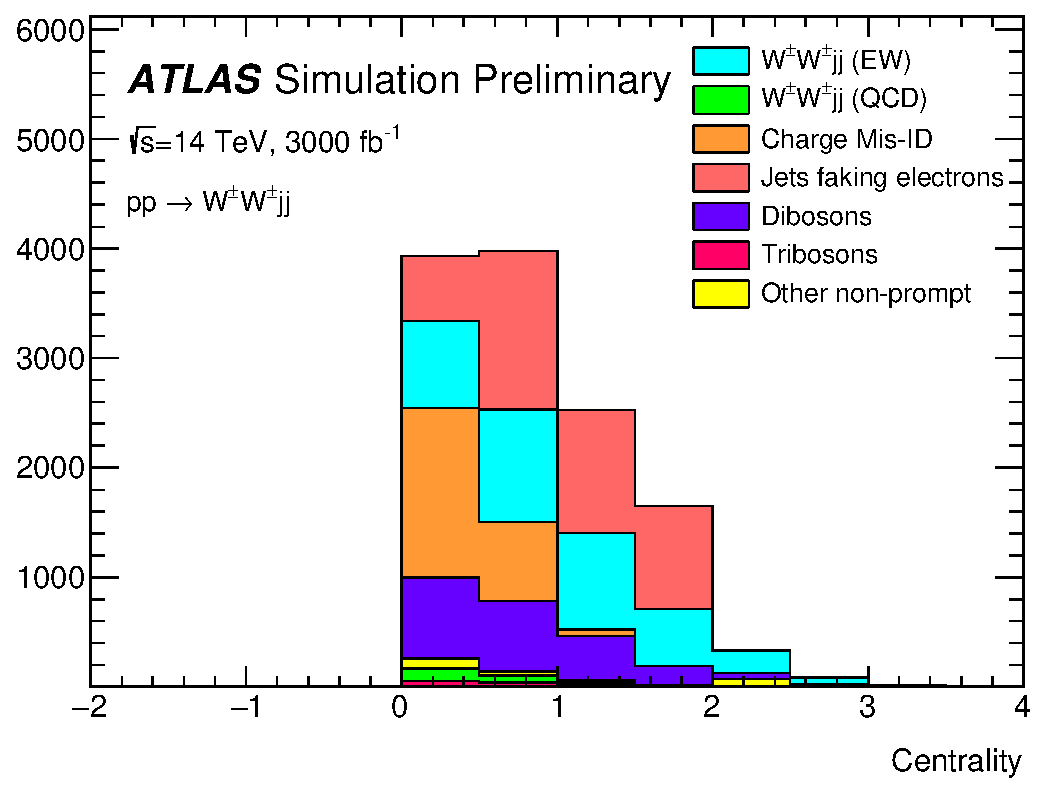
\includegraphics[width=\textwidth]{figs/ssww_upgrade/distributions/default/all_pass9_lepjet_centrality-cropped}
    \caption{Default selection}
    \label{fig:sswwupgrade_centrality_compare_d}
  \end{subfigure}
  \begin{subfigure}[b]{.4792\textwidth}
  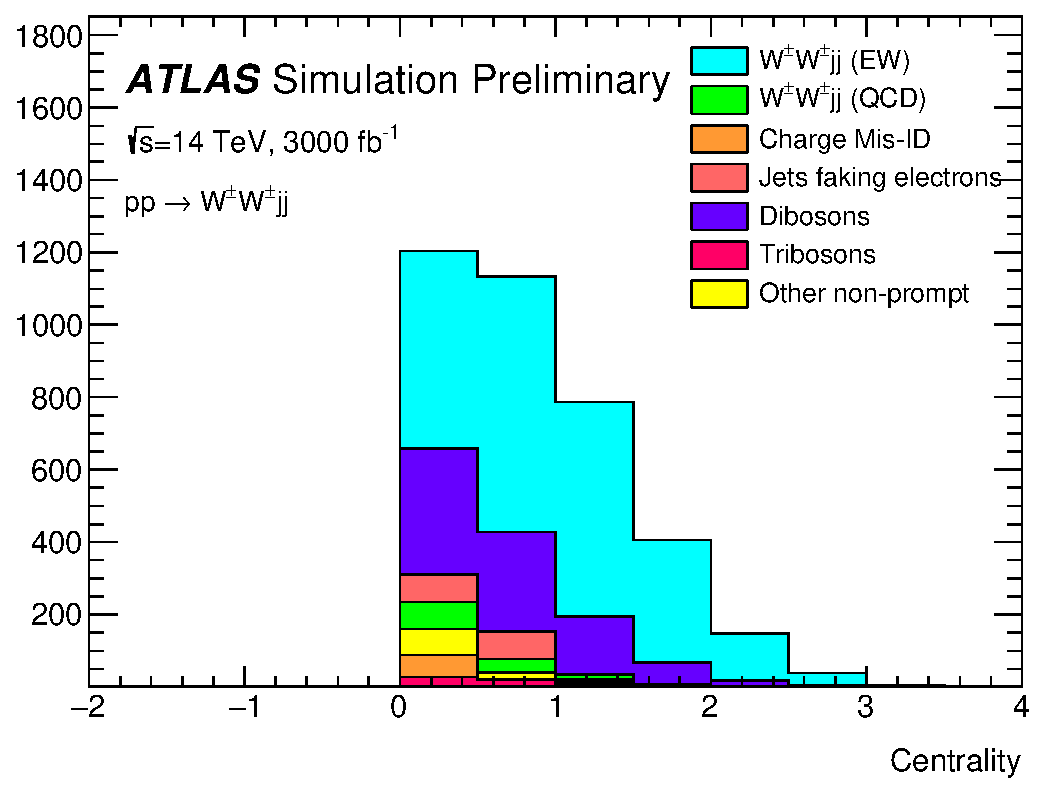
\includegraphics[width=\textwidth]{figs/ssww_upgrade/distributions/optimized/all_pass9_lepjet_centrality-cropped}
    \caption{Optimized selection}
    \label{fig:sswwupgrade_centrality_compare_o}
  \end{subfigure}
  \caption{$\pt$ distributions for lepton-jet centrality $\zeta$ using the default (left) and optimized (right) event selections for all channels combined.}
  \label{fig:sswwupgrade_centrality_compare}
\end{figure}

It is important to note, however, that the MC sample used to estimate $Z$+jets events suffers from poor statistics which results in large per-event weights once scaled to $\mathcal{L} = 3000~\textrm{fb}^{-1}$.
This sample contributes heavily to the fake and charge misidentification backgrounds, and a handful of these events being cut out by the optimization is largely responsible for the dramatic reduction of the corresponding backgrounds.
As a result, the optimized results presented here are likely overly optimistic.
However, given proper MC statistics, it is still expected that this optimization will outperform the default selection.

\subsection{Uncertainties}\label{sswwupgrade:results_uncertainties}
%\TODO{Ask for details on how some of these uncertainties were calculated -- specifically the fakes and charge mis-ID}
The uncertainties considered for the analysis are summarized in Table~\ref{tab:sswwupgrade_uncertainties}.
Values for experimental systematics on the trigger efficiency, lepton and jet reconstruction, and flavor tagging are taken directly from the $13\tev$ analysis \cite{2018.ssww-13tev-paper-draft}.
The rate uncertainties for the background processes are halved from the $13\tev$ values according to ATLAS recommendations.
The uncertainty on the fake electron estimation is also halved from the $13\tev$ analysis.
Finally, a conservative estimate of the uncertainty on the charge flip background is used as the electron charge mis-ID rate due to material interactions is difficult to predict at this stage. 

\begin{table}[htbp]
  \centering
  \begin{tabular}{l|c}
    Source	& Uncertainty (\%) \\
    \hline\hline
    \ssww (EWK)	&   3 \\
    \hline
    Luminosity			&  1 \\
    \hline
    Trigger efficiency & 0.5 \\
    Lepton reconstruction and identification	&  1.8\\
    Jets &  2.3\\
    Flavor tagging	&  1.8\\
    \hline
    Jets faking electrons	&  20\\
    Charge misidentification	&  25\\
    \hline
    \ssww (QCD)	&  20\\
    Top	&  15 \\
    Diboson	&   10 \\
    Triboson	&   15 \\
    \hline\hline
  \end{tabular}
  \caption{Summary of estimated experimental and rate uncertainties.}
  \label{tab:sswwupgrade_uncertainties}
\end{table}

\subsection{Cross section measurement}\label{sswwupgrade:results_xsec}

The cross section is calculated using the same method as in the $13\tev$ analysis, detailed in Section~\ref{ssww13tev:xsec}.
Unlike the previous analysis, however, eight lepton channels are used here instead of six.
The $\mu e$ and $e\mu$ channels remain separated in addition to the $\mu\mu$ and $ee$ channels, and each lepton flavor channel is further split by charge, as this increases the sensitivity of the analysis.
Each channel's $m_{jj}$ distribution is combined in a profile likelihood fit to extract the EWK \ssww production cross section.
Using the default event selection, the expected cross section calculated to be
\begin{equation}
  \sigma_{W^\pm W^\pm jj}^{\textrm{expected}} = 16.89 \pm 0.36 \textrm{\ (stat)} \pm 0.53 \textrm{\ (theory)} \pm 0.84 \textrm{\ (syst)}~\textrm{fb}\,.
  \label{eq:sswwupgrade_xsec_default}
\end{equation}
With the optimized event selection, the expected cross section is
\begin{equation}
    \sigma_{W^\pm W^\pm jj}^{\textrm{expected}} = 16.94 \pm 0.36 \textrm{\ (stat)} \pm 0.53 \textrm{\ (theory)} \pm 0.78 \textrm{\ (syst)}~\textrm{fb}\,.
  \label{eq:sswwupgrade_xsec_optimized}
\end{equation}
The optimized selection should not change the measured value of the cross section, and indeed both are consistent with within uncertainties.
The systematic uncertainty is reduced by about 7\% with the optimized selection.
The total uncertainty on the cross section measurement is approximately $6\%$, compared to the $20\%$ uncertainty on the measured fiducial cross section of the $13\tev$ analysis reported in Equation~\ref{eq:ssww13tev_fiducial_xsec}.

Projections of each uncertainty type and the total uncertainty on the cross section as a function of integrated luminosity are shown in Figure~\ref{fig:sswwupgrade_uncertainty_projection}.
The predictions are made by scaling the event yields by different luminosity values and re-running the fitting procedure.
As the integrated luminosity increases past $\mathcal{L} > 3000~\textrm{fb}^{-1}$, the statistical uncertainty continues to reduce; however, the total uncertainty will be limited by the systematics.
%Additionally, the total uncertainty is expected to reduce by less than a percent as the integrated luminosity increases past the planned $3000~\textrm{fb}^{-1}$.
The end result is that after collecting the planned $3000~\textrm{fb}^{-1}$, the precision the \ssww cross section measurement is expected to be more than a factor of three better than in the $13\tev$ analysis, with diminishing returns with additional data.

\begin{figure}[htbp]
  \centering
  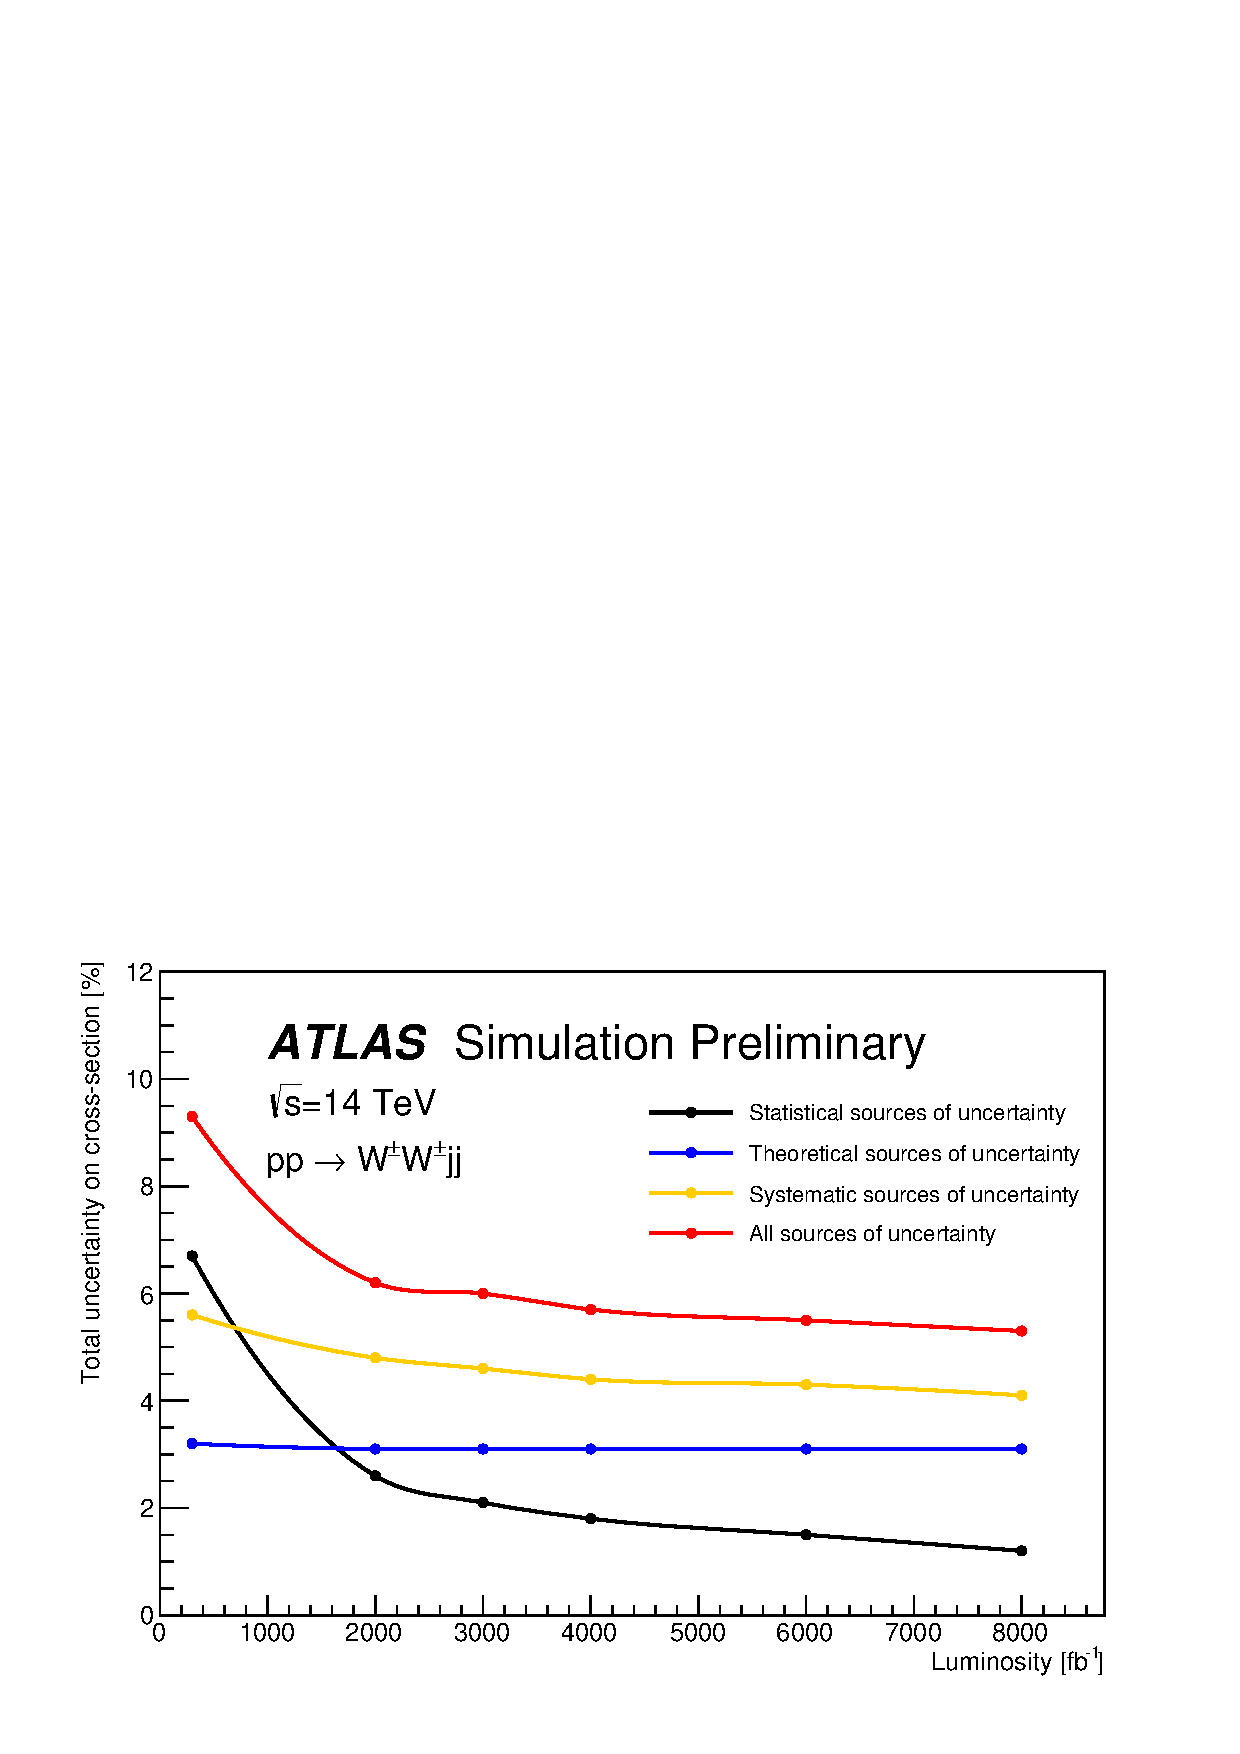
\includegraphics[width=.8\textwidth]{figs/ssww_upgrade/results/uncertainty_projection}
  \caption{Projections of the statistical (black), theoretical (blue), systematic (yellow), and total (red) uncertainties on the measured cross section as a function of integrated luminosity using the optimized event selection.}
  \label{fig:sswwupgrade_uncertainty_projection}
\end{figure}

\subsection{Longitudinal scattering significance}\label{sswwupgrade:results_longitudinal_sig}
The longitudinal scattering significance is extracted in much the same way as the cross section, this time using a binned likelihood fit on the $|\dphijj|$ distribution.
In order to increase sensitivity, the $|\dphijj|$ distribution is split into two bins in $m_{jj}$, and an additional cut on the pseudorapidity of the subleading lepton is applied ($|\eta| < 2.5$) to reduce background contributions from fake electrons and charge flip.
The $|\dphijj|$ distributions used in the fit are shown in Figure~\ref{fig:sswwupgrade_dphijj_LL}.
Due to limited statistics in the LL events, the four lepton flavor channels are not split by charge.
The expected significance of the \sswwll process is $1.8\sigma$ with a precision of $47\%$ on the measurement.
Projections of the expected significance as a function of integrated luminosity is shown in Figure~\ref{fig:sswwupgrade_LL_significance_projection}, and once again, the improvement in the precision with additional data becomes small after the initial $3000~\textrm{fb}^{-1}$.
%\TODO{Ask Karolos how the expected significance vs luminosity plot was made!}

\begin{figure}[htbp]
  \centering
  \begin{subfigure}[b]{.48\textwidth}
    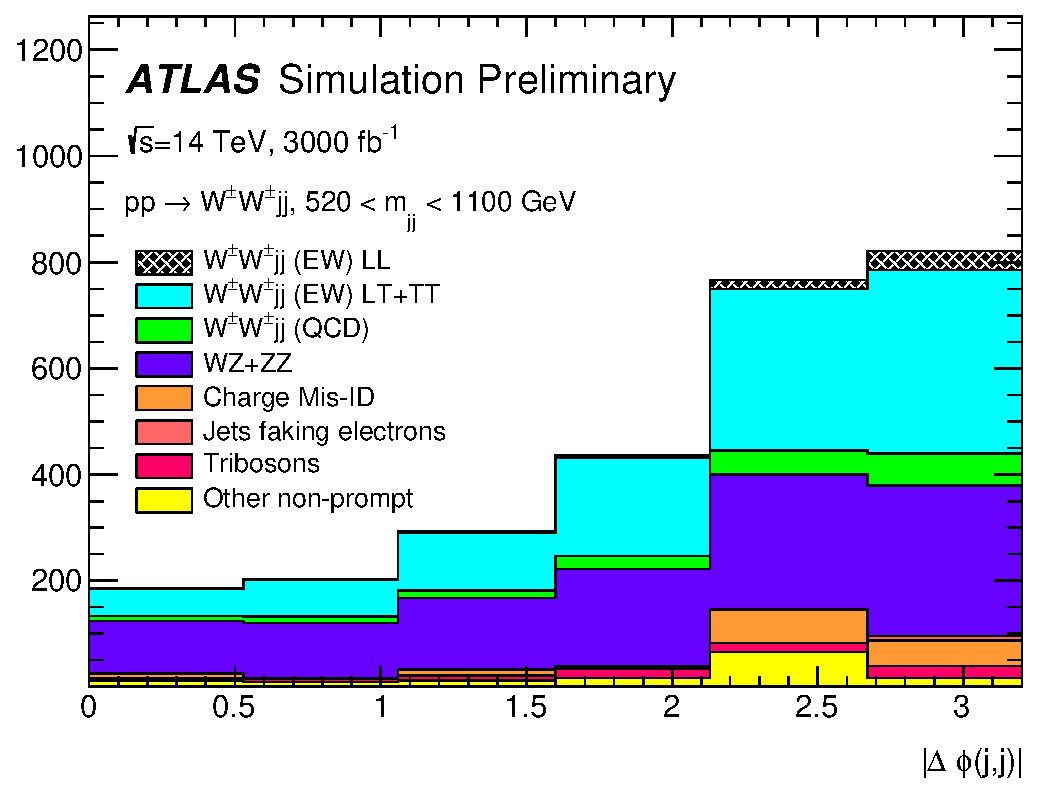
\includegraphics[width=\textwidth]{figs/ssww_upgrade/results/plots_optimisedLL_all_pass9_dijet_absdphijj_lowmjj-cropped}
    \caption{Low $m_{jj}$ bin ($520 < m_{jj} < 1100\gev$)}
    \label{fig:sswwupgrade_dphijj_LL_low}
  \end{subfigure}
  \begin{subfigure}[b]{.48\textwidth}
    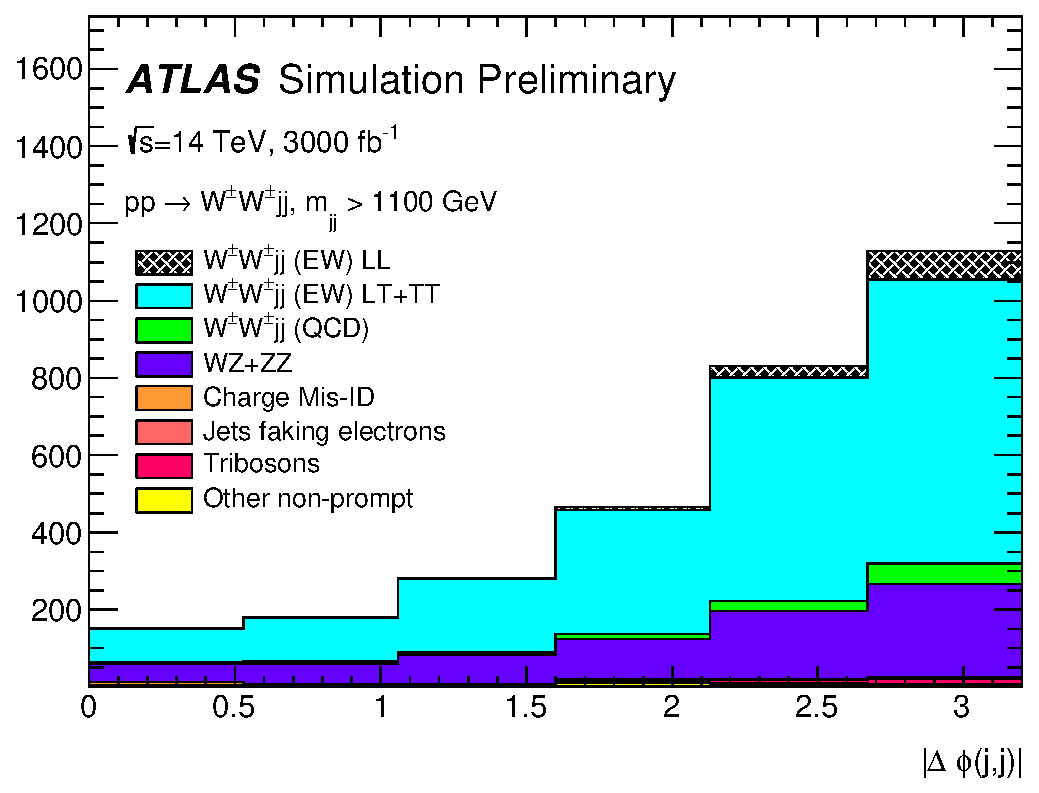
\includegraphics[width=\textwidth]{figs/ssww_upgrade/results/plots_optimisedLL_all_pass9_dijet_absdphijj_highmjj-cropped}
    \caption{High $m_{jj}$ bin ($m_{jj} > 1100\gev$)}
    \label{fig:sswwupgrade_dphijj_LL_high}
  \end{subfigure}
  \caption{Dijet azimuthal separation ($|\dphijj|$) for the low $m_{jj}$ region ($520 < m_{jj} < 1100\gev$, top) and the high $m_{jj}$ region ($m_{jj} > 1100\gev$, bottom).  The purely longitudinal (LL, gray) is plotted separately from the mixed and transverse (LT+TT, cyan) polarizations.}
  \label{fig:sswwupgrade_dphijj_LL}
\end{figure}

\begin{figure}[htbp]
  \centering
  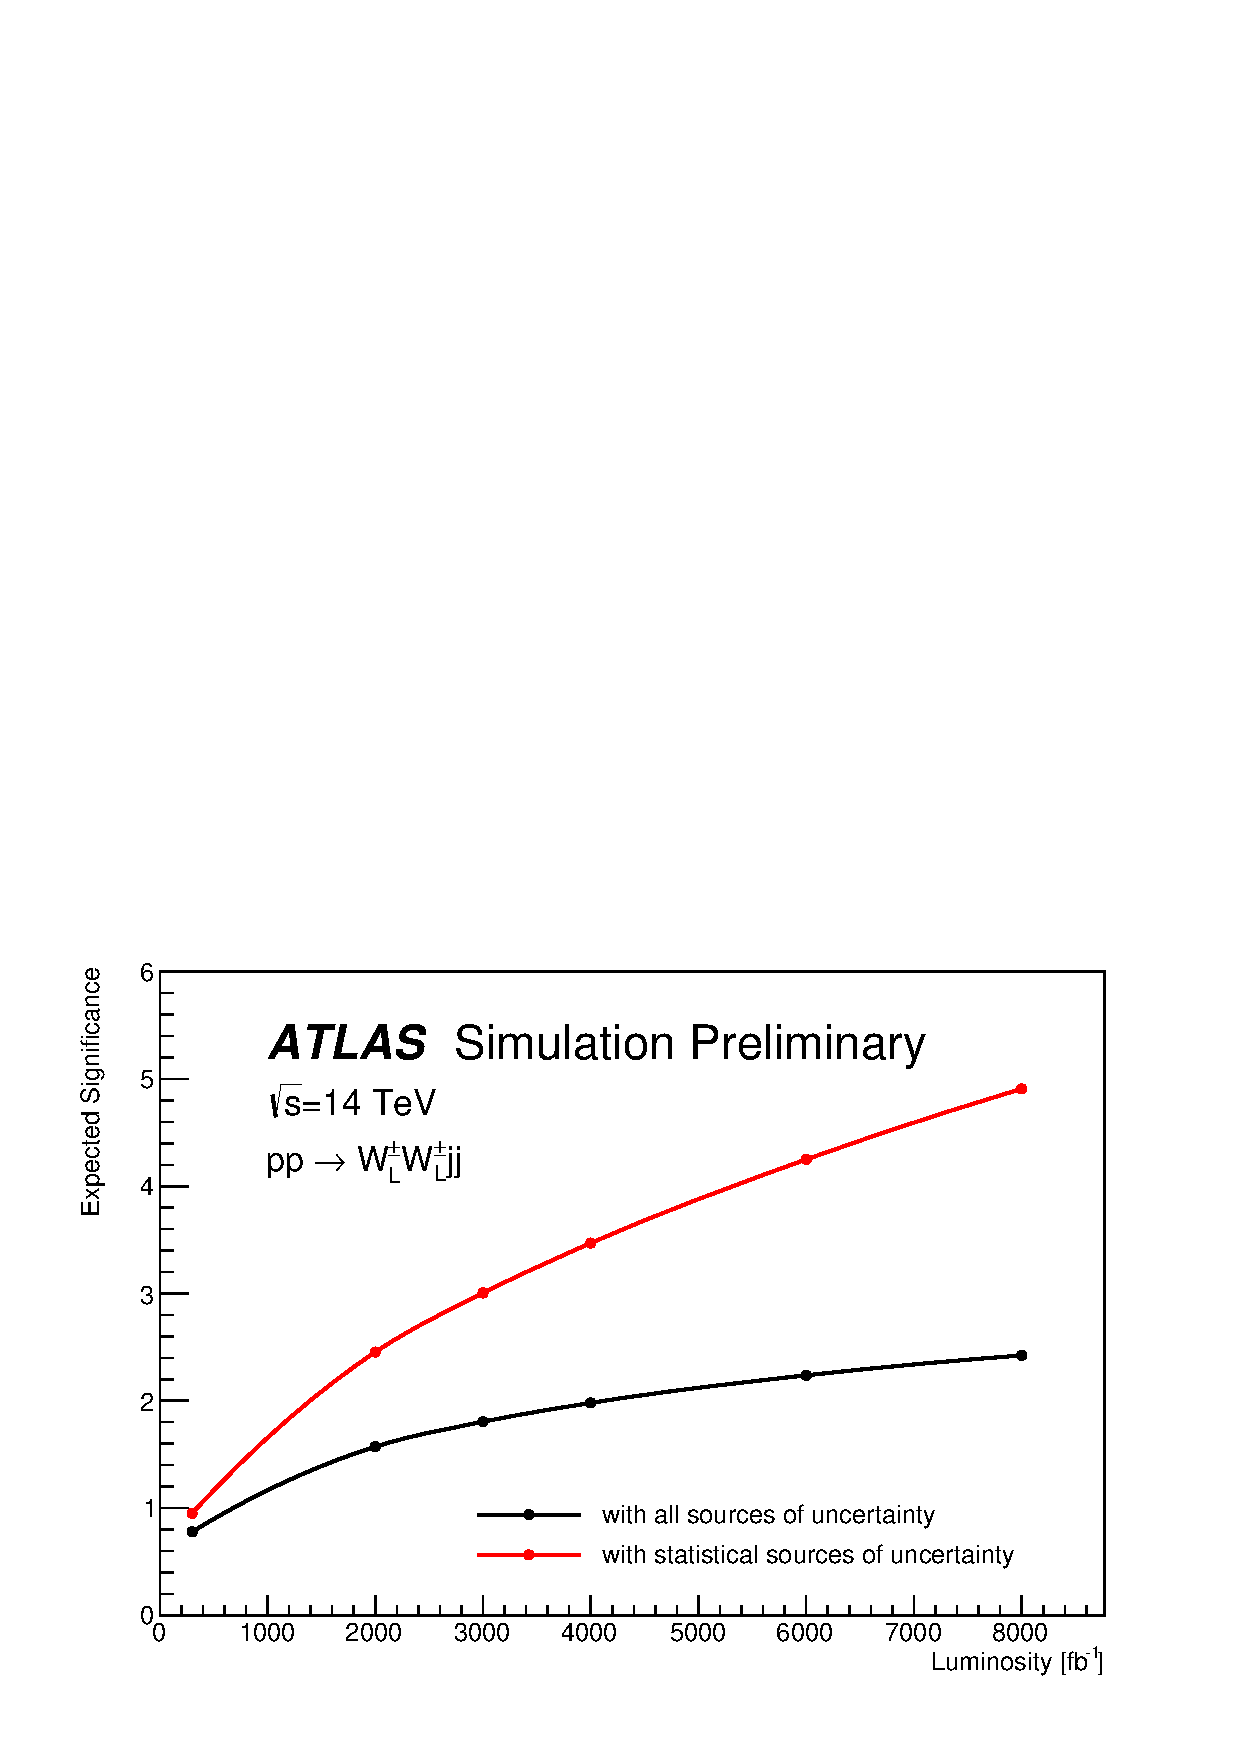
\includegraphics[width=.8\textwidth]{figs/ssww_upgrade/results/LLsignificance_projection}
  \caption{Projections of the expected longitudinal scattering significance as a function of integrated luminosity when considering all sources of uncertainties (black) or only statistical uncertainties (red).}
  \label{fig:sswwupgrade_LL_significance_projection}
\end{figure}
